\chapter{Arquitectura final de TierraViva}
\label{cap:capitulo4}

Una vez definidos los requisitos, los materiales y las principales decisiones de diseño, este capítulo presenta la arquitectura final de TierraViva. A diferencia del capítulo anterior, donde se justifican las alternativas valoradas y los criterios de elección, aquí se describe cómo queda organizado el sistema completo y cómo interactúan sus distintos bloques durante el funcionamiento.

La arquitectura final se basa en estaciones de campo autónomas con Arduino UNO, sensores ambientales y de suelo, comunicación LTE mediante el módulo A7670E-LASA, una plataforma cloud intermedia basada en ThingSpeak y un sistema de supervisión implementado sobre Raspberry Pi 5. El sistema se ha diseñado para cubrir el ciclo completo de monitorización y actuación local: adquisición de datos, decisión de riego en la estación, actuación sobre la bomba, publicación de telemetría y estado, almacenamiento histórico, API y visualización mediante dashboard web.

El cambio principal respecto a planteamientos anteriores es que la Raspberry Pi no actúa como elemento central de decisión del riego. La decisión crítica se desplaza al firmware de cada estación, que evalúa sus propias lecturas y aplica reglas locales de seguridad. La Raspberry conserva un papel importante, pero orientado a supervisión, histórico y visualización.

\section{Visión general de la arquitectura}
\label{sec:vision_general_arquitectura}

La arquitectura final de TierraViva se organiza como un sistema IoT distribuido. Las medidas se obtienen en campo, la comunicación se realiza mediante red móvil, la información se publica en una plataforma cloud y la supervisión se ejecuta desde una Raspberry Pi 5. La actuación sobre el riego, sin embargo, no depende de una decisión externa enviada desde la Raspberry, sino de reglas locales ejecutadas en cada estación.

El sistema está formado por cuatro elementos principales: las estaciones autónomas de campo A y B, la plataforma ThingSpeak, la Raspberry Pi 5 y el dashboard web. Las estaciones se encargan de medir, decidir y actuar localmente. ThingSpeak funciona como capa intermedia de telemetría y estado. La Raspberry Pi consulta los datos, mantiene un histórico local y expone una API. El dashboard permite supervisar el estado del sistema desde una interfaz web.

La Figura~\ref{fig:arquitectura_final_tierraviva} muestra la arquitectura final del sistema.

\begin{figure}[H]
\centering
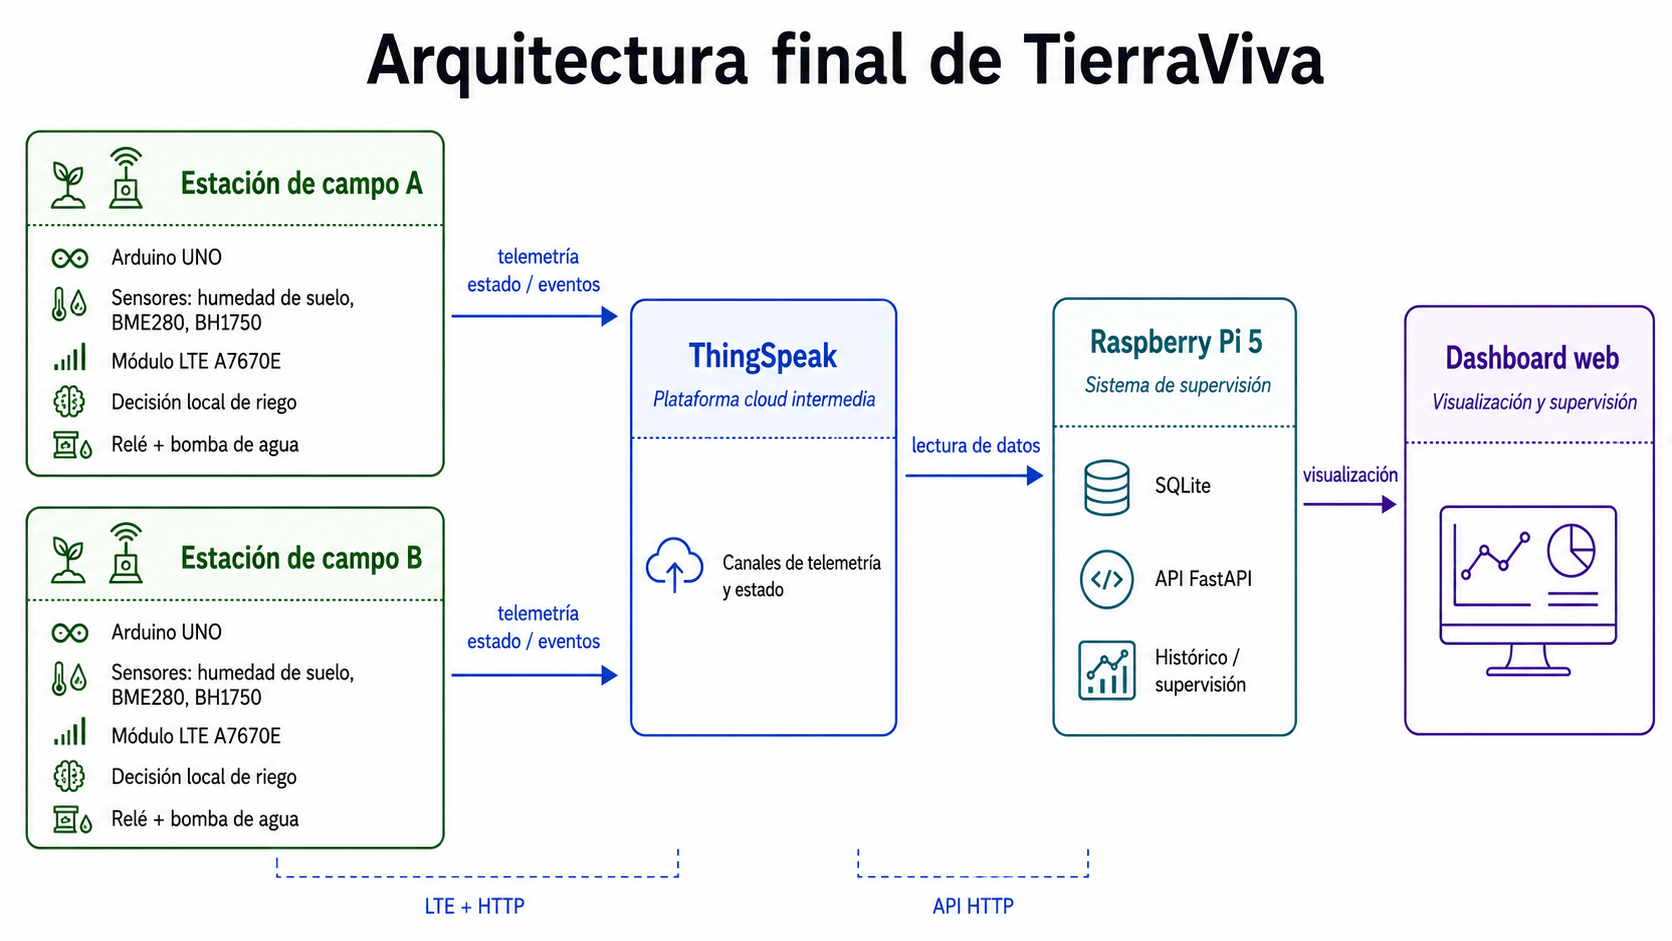
\includegraphics[width=\textwidth]{figs/arquitecturaFinalTierraViva.png}
\caption{Arquitectura final de TierraViva con decisión local en las estaciones.}
\label{fig:arquitectura_final_tierraviva}
\end{figure}

El flujo de funcionamiento comienza en las estaciones de campo. Cada estación toma lecturas de sus sensores, evalúa localmente si se cumplen las condiciones de riego y, si procede, activa la bomba de agua mediante el relé durante un tiempo limitado. Después publica en ThingSpeak tanto las medidas ambientales como el estado del relé y el código de estado correspondiente.

ThingSpeak actúa como punto de desacoplo entre los nodos de campo y el sistema de supervisión. Las estaciones no necesitan conocer la ubicación de la Raspberry ni mantener una conexión directa con ella; únicamente publican información en la nube. La Raspberry, por su parte, consulta periódicamente los canales de ThingSpeak y almacena los datos relevantes en su base de datos local.

La Raspberry Pi 5 funciona como sistema de supervisión. Su papel no es accionar directamente la bomba, leer sensores por cable ni decidir cuándo debe regarse. Su función es consultar la telemetría disponible, registrar el histórico en SQLite, exponer los datos mediante una API y servir el dashboard web. Así, una caída de la Raspberry no impide que la estación mantenga su comportamiento local de seguridad.

El dashboard web representa la capa de visualización. A partir de la información procesada por la Raspberry Pi, permite consultar las últimas lecturas, el estado de las estaciones, el estado del relé y los estados de funcionamiento publicados por cada nodo. No participa directamente en la actuación, pero resulta fundamental para supervisar el comportamiento del prototipo y detectar posibles incidencias.

La arquitectura final puede resumirse de forma sencilla: las estaciones miden, deciden y actúan en campo; ThingSpeak comunica y almacena telemetría; la Raspberry registra y supervisa; y el dashboard permite visualizar. Esta organización facilita la validación por bloques, permite trabajar con más de una estación y mantiene una separación clara entre adquisición, comunicación, decisión local, actuación y supervisión.

\section{Estaciones de campo A y B}
\label{sec:estaciones_campo_ab}

Las estaciones de campo son los nodos autónomos de TierraViva. Su función dentro de la arquitectura final es adquirir datos del entorno, evaluar localmente reglas de riego, accionar la bomba cuando corresponda y publicar telemetría y estado en la plataforma cloud. En esta versión del sistema se contemplan dos estaciones, denominadas estación A y estación B, con una estructura hardware equivalente y una configuración lógica diferenciada.

Ambas estaciones siguen el mismo diseño base: Arduino UNO como controlador local, sensores de suelo y ambientales, módulo LTE A7670E-LASA para comunicación remota, relé para accionar la bomba de agua y alimentación principal a 12 V con regulación a 5 V mediante LM2596. La diferencia entre ellas no está en la arquitectura física, sino en el identificador de estación y el canal de ThingSpeak utilizado para publicar sus datos.

\begin{table}[H]
\begin{center}
\small
\begin{tabular}{|p{0.26\textwidth}|p{0.30\textwidth}|p{0.34\textwidth}|}
\hline
\textbf{Elemento} & \textbf{Estación A} & \textbf{Estación B} \\
\hline
Identificador lógico & \texttt{TierraViva\_A} & \texttt{TierraViva\_B} \\
\hline
Controlador local & Arduino UNO & Arduino UNO \\
\hline
Sensores & Humedad de suelo, BME280 y BH1750 & Humedad de suelo, BME280 y BH1750 \\
\hline
Comunicación & A7670E-LASA mediante LTE/HTTP & A7670E-LASA mediante LTE/HTTP \\
\hline
Canal ThingSpeak & Canal asociado a estación A & Canal asociado a estación B \\
\hline
Decisión de riego & Regla local en firmware & Regla local en firmware \\
\hline
Actuación & Relé y bomba de agua 12 V & Relé y bomba de agua 12 V \\
\hline
Alimentación & 12 V con regulación a 5 V & 12 V con regulación a 5 V \\
\hline
\end{tabular}
\caption{Configuración lógica de las estaciones de campo}
\label{cuadro:configuracion_estaciones}
\end{center}
\end{table}

La Tabla~\ref{cuadro:configuracion_estaciones} resume esta configuración. El objetivo de mantener estaciones equivalentes es facilitar la reproducción del sistema: una vez validada la estación A, la estación B puede construirse replicando el mismo montaje y modificando únicamente los parámetros de identificación y comunicación. Esta decisión también simplifica la depuración, ya que cualquier diferencia de comportamiento entre estaciones puede analizarse a partir de una base hardware común.

Desde el punto de vista interno, cada estación se organiza en cuatro bloques funcionales. El primero es el bloque de adquisición, formado por el sensor capacitivo de humedad del suelo, el BME280 y el BH1750. El segundo es el bloque de decisión local, ejecutado en el firmware del Arduino. El tercero es el bloque de comunicación, formado por el A7670E-LASA y la lógica de publicación mediante HTTP. El cuarto es el bloque de actuación, formado por la salida digital del Arduino, el módulo relé y la bomba de agua de 12 V.

\begin{table}[H]
\begin{center}
\small
\begin{tabular}{|p{0.25\textwidth}|p{0.32\textwidth}|p{0.33\textwidth}|}
\hline
\textbf{Bloque interno} & \textbf{Elementos implicados} & \textbf{Responsabilidad} \\
\hline
Adquisición & Sensores y Arduino UNO & Obtener lecturas periódicas del suelo y del entorno. \\
\hline
Decisión local & Arduino UNO & Evaluar humedad del suelo, cooldown, errores y condiciones de seguridad. \\
\hline
Comunicación & Arduino UNO y A7670E-LASA & Publicar telemetría, estado y eventos en ThingSpeak. \\
\hline
Actuación & Arduino UNO, relé y bomba & Ejecutar el riego localmente durante un tiempo limitado. \\
\hline
Alimentación & Fuente 12 V, LM2596 y condensadores & Proporcionar tensión adecuada y estabilidad eléctrica al montaje. \\
\hline
\end{tabular}
\caption{Bloques internos de una estación de campo}
\label{cuadro:bloques_internos_estacion}
\end{center}
\end{table}

El firmware de estación debe mantener esta separación de responsabilidades. En primer lugar, realiza la lectura de sensores y genera una estructura de datos con las variables medidas. Después, comprueba si las lecturas son válidas y evalúa la regla local de riego. Si la humedad del suelo indica sequedad, no existe cooldown activo y no se detecta una condición de error, la estación puede activar el relé durante el tiempo máximo configurado.

La actuación se ejecuta siempre de forma local. Cuando una estación decide regar, activa el relé durante un tiempo limitado y posteriormente vuelve a dejar la bomba apagada. Durante las pruebas iniciales puede utilizarse una carga de baja potencia, como un LED, para comprobar la lógica de activación sin accionar todavía la bomba real. En el montaje final, esa carga de prueba se sustituye por la bomba de agua de 12 V.

La estación conserva la responsabilidad última sobre la ejecución segura. Antes de activar el relé debe comprobar que la lectura de humedad es válida, que la duración máxima no se supera, que no existe un error crítico y que no se está dentro del periodo mínimo entre riegos. Si alguna de estas comprobaciones falla, la estación mantiene la bomba apagada y publica un código de estado que permita diagnosticar la situación desde la Raspberry Pi.

La alimentación de cada estación parte de una tensión principal de 12 V, necesaria para el bloque de actuación. A partir de esa tensión se obtiene una línea de 5 V mediante el regulador LM2596 para alimentar la electrónica compatible. En el montaje se incorporan condensadores de estabilización para reducir inestabilidades asociadas a consumos variables, especialmente durante la comunicación LTE o los cambios de estado del bloque de actuación. El detalle de conexiones eléctricas se recoge en el Anexo~\ref{anexo:esquemas_conexion}.

En resumen, las estaciones A y B son nodos de campo equivalentes desde el punto de vista hardware, pero diferenciados por configuración. Esta organización permite escalar el sistema sin rediseñar la arquitectura: añadir una nueva estación implicaría replicar el montaje, asignar un nuevo identificador, crear un nuevo canal de ThingSpeak y ajustar la lógica de supervisión para consultar ese nuevo origen de datos.

\section{Arquitectura de comunicaciones LTE/HTTP}
\label{sec:arquitectura_comunicaciones_lte_http}

La comunicación de las estaciones de campo se basa en el módulo LTE A7670E-LASA y en el uso de peticiones HTTP hacia ThingSpeak. Esta arquitectura permite que cada estación publique telemetría y estado desde una ubicación remota sin depender de una red WiFi local ni de una conexión física con la Raspberry Pi. Desde el punto de vista funcional, el módulo LTE actúa como interfaz de salida a Internet de la estación.

El Arduino UNO no accede directamente a la red móvil. Su papel es comunicarse por UART con el A7670E-LASA mediante comandos AT. A través de esa interfaz serie, el firmware comprueba el estado del módulo, verifica la SIM, confirma el registro en red, configura el contexto de datos y lanza las peticiones HTTP necesarias para enviar información a la nube. Esta separación permite que el Arduino mantenga una lógica relativamente sencilla: preparar datos, aplicar la decisión local, enviarlos al módem y analizar la respuesta obtenida.

El flujo de comunicación se organiza en varias fases. La primera corresponde a la inicialización del módulo. En esta fase, la estación comprueba que el A7670E-LASA responde a comandos básicos y que la comunicación serie funciona correctamente. Después, se verifica el estado de la SIM y el registro en la red móvil. Una estación no debería intentar enviar telemetría si el módulo no responde, si la SIM no está preparada o si no existe registro válido en red.

A continuación, se configura el contexto de datos. Para ello, el módulo debe disponer de un APN válido asociado a la tarjeta SIM utilizada. Este paso es necesario para que el módem pueda obtener conectividad IP. Una vez configurado el contexto y obtenida una dirección IP, la estación puede iniciar la secuencia HTTP.

La fase de envío consiste en construir una URL de actualización de ThingSpeak con los campos de telemetría correspondientes. Cada estación incluye sus medidas y estados en los campos definidos para su canal: humedad de suelo, temperatura, humedad relativa, luminosidad, presión, estado del relé, código de estado o evento y un campo auxiliar de diagnóstico. El A7670E-LASA realiza entonces una petición HTTP hacia la API de ThingSpeak.

\begin{table}[H]
\begin{center}
\small
\begin{tabular}{|p{0.22\textwidth}|p{0.31\textwidth}|p{0.35\textwidth}|}
\hline
\textbf{Fase} & \textbf{Acción principal} & \textbf{Resultado esperado} \\
\hline
Inicialización & Comprobar comunicación con el módulo mediante comandos AT. & El módulo responde correctamente y queda listo para continuar. \\
\hline
SIM & Verificar que la tarjeta SIM está disponible y sin PIN pendiente. & La SIM se encuentra preparada para registrarse en red. \\
\hline
Registro en red & Comprobar el registro LTE y la calidad de señal. & La estación confirma que existe cobertura móvil suficiente. \\
\hline
Contexto de datos & Configurar APN y comprobar dirección IP. & El módulo dispone de conectividad IP para realizar peticiones. \\
\hline
Envío HTTP & Construir la petición de actualización y enviarla a ThingSpeak. & La plataforma recibe una nueva entrada de telemetría y estado. \\
\hline
Gestión de respuesta & Analizar el código de respuesta y cerrar la sesión HTTP. & La estación confirma si el envío ha sido correcto o registra un error. \\
\hline
\end{tabular}
\caption{Fases de comunicación LTE/HTTP en una estación de campo}
\label{cuadro:fases_lte_http}
\end{center}
\end{table}

La Tabla~\ref{cuadro:fases_lte_http} resume el flujo seguido por la estación. Esta secuencia no se ejecuta únicamente como una lista fija de comandos AT, sino como una lógica de comunicación con comprobaciones intermedias. Si una fase falla, el firmware debe evitar continuar como si el envío hubiera sido correcto. Por ejemplo, no tiene sentido construir una petición HTTP si el módulo no está registrado en red o si no dispone de dirección IP.

En la comunicación con ThingSpeak se utiliza el modelo HTTP de petición-respuesta. La estación envía una petición de escritura al canal correspondiente y espera una respuesta de la plataforma. En un envío correcto, ThingSpeak devuelve una confirmación que permite interpretar que la entrada ha sido registrada. Si la respuesta indica error, si no llega respuesta o si se agota el tiempo de espera, la estación debe tratar el envío como fallido.

La gestión de errores forma parte de la propia arquitectura de comunicaciones. Los fallos posibles no se limitan a una ausencia total de cobertura. También pueden aparecer reinicios del módulo por alimentación insuficiente, errores de APN, pérdida temporal de red, fallo de resolución o respuesta HTTP no válida. Por ello, el firmware debe diferenciar entre un dato no enviado y una actuación física sobre el riego. La pérdida temporal de comunicación puede impedir la supervisión remota, pero no debe dejar la bomba activa ni provocar una actuación no controlada.

La comunicación LTE/HTTP se emplea únicamente en sentido ascendente desde el punto de vista operativo de la estación: publicación de telemetría, estado y eventos. La Raspberry Pi realiza después lecturas de esos datos desde ThingSpeak, pero no envía órdenes de riego a las estaciones. Esta decisión simplifica el firmware, evita un flujo descendente de control y reduce el riesgo de que información antigua en la nube condicione una actuación física.

Esta arquitectura no proporciona comunicación en tiempo real estricto. La estación publica información de forma periódica, por lo que existe una latencia asociada a los intervalos de muestreo y envío. Sin embargo, para supervisión de riego esta latencia es aceptable. La decisión crítica no depende de la llegada inmediata de una orden externa, sino de la evaluación local realizada en la propia estación.

En conjunto, la arquitectura LTE/HTTP permite que las estaciones funcionen como nodos remotos independientes del sistema de supervisión físico. Cada estación puede publicar sus datos en la nube, mantener una lógica local de riego y permitir que la Raspberry Pi consulte posteriormente el estado del sistema sin conexión directa con el hardware de campo.

\section{ThingSpeak como capa intermedia}
\label{sec:thingspeak_capa_intermedia}

ThingSpeak actúa en TierraViva como capa intermedia entre las estaciones de campo y la Raspberry Pi. Su función dentro de la arquitectura final es desacoplar la publicación de datos en campo de la supervisión posterior: las estaciones publican telemetría y estado mediante LTE/HTTP, mientras que la Raspberry Pi lee esa información, mantiene un histórico local y la muestra en el dashboard.

La estructura finalmente adoptada se apoya en dos canales diferenciados: \texttt{TierraViva\_A} y \texttt{TierraViva\_B}. Cada canal corresponde a una estación de campo y contiene tanto las variables medidas como la información de estado generada por el firmware. En la arquitectura final no se utilizan canales de comandos, ya que la decisión de riego se realiza localmente en cada estación.

La Figura~\ref{fig:thingspeak_canales_tierraviva} muestra los canales creados en ThingSpeak para el prototipo.

\begin{figure}[H]
\centering
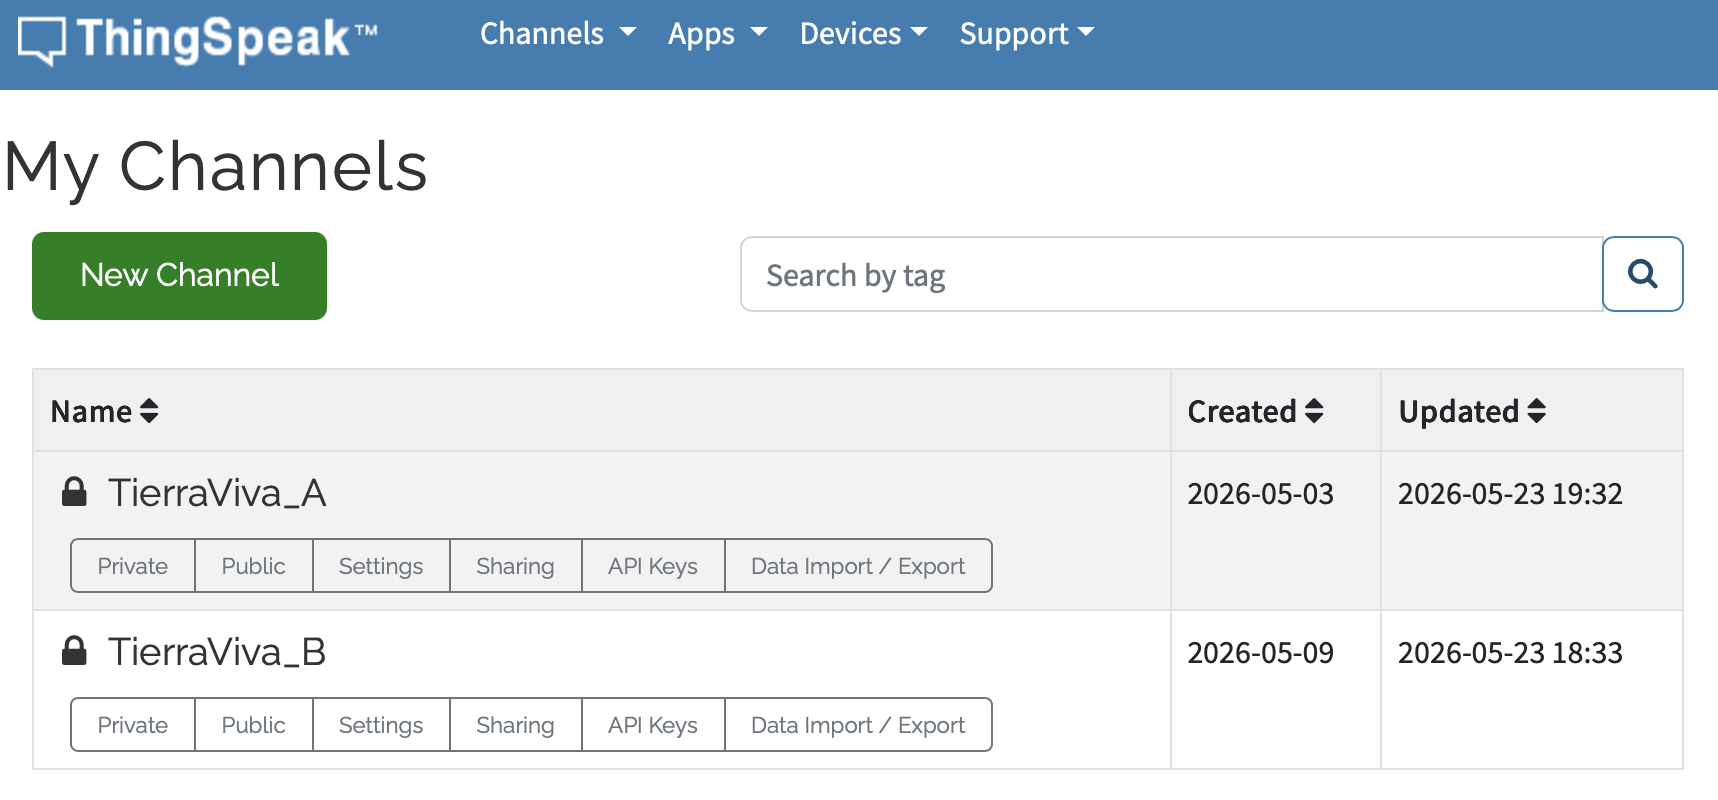
\includegraphics[width=0.90\textwidth]{figs/thingspeak_canales_tierraviva.png}
\caption{Canales ThingSpeak creados para las estaciones de TierraViva.}
\label{fig:thingspeak_canales_tierraviva}
\end{figure}

\subsection{Canales de estación}
\label{subsec:canales_estacion}

Los canales \texttt{TierraViva\_A} y \texttt{TierraViva\_B} almacenan la telemetría generada por las estaciones A y B, respectivamente. Cada actualización enviada por una estación incluye medidas del entorno y datos de estado, lo que permite a la Raspberry Pi supervisar tanto las variables ambientales como el comportamiento operativo del nodo.

\begin{table}[H]
\begin{center}
\small
\begin{tabular}{|p{0.18\textwidth}|p{0.28\textwidth}|p{0.44\textwidth}|}
\hline
\textbf{Campo} & \textbf{Dato} & \textbf{Descripción} \\
\hline
\texttt{field1} & Humedad del suelo normalizada (\%) & Valor calculado por el firmware a partir de la lectura bruta del sensor capacitivo. Se utiliza como entrada principal de la regla local de riego. \\
\hline
\texttt{field2} & Temperatura (\textdegree C) & Temperatura ambiente medida por el BME280. \\
\hline
\texttt{field3} & Humedad ambiente (\%) & Humedad relativa medida por el BME280. \\
\hline
\texttt{field4} & Luminosidad (lux) & Nivel de luz ambiente medido por el BH1750. \\
\hline
\texttt{field5} & Presión (hPa) & Presión atmosférica medida por el BME280. \\
\hline
\texttt{field6} & Estado del relé & Estado del relé asociado al bloque de actuación: \texttt{0} para apagado y \texttt{1} para activo. \\
\hline
\texttt{field7} & Modo seguro & Indicador de seguridad de la estación: \texttt{0} para funcionamiento normal y \texttt{1} para modo seguro activo. \\
\hline
\texttt{field8} & Código de estado & Código numérico que resume el estado operativo del ciclo o la incidencia detectada. \\
\hline
\end{tabular}
\caption{Asignación de campos en los canales ThingSpeak de estación}
\label{cuadro:canales_thingspeak_estacion}
\end{center}
\end{table}

La Tabla~\ref{cuadro:canales_thingspeak_estacion} define el contrato de datos utilizado por las estaciones. Mantener la misma estructura en ambos canales simplifica el firmware y la lógica de supervisión, ya que la Raspberry puede aplicar el mismo proceso de lectura para la estación A y para la estación B, cambiando únicamente el identificador del canal y la clave de lectura correspondiente.

Esta estructura permite que el canal no se limite a representar medidas ambientales. En particular, los campos \texttt{field6}, \texttt{field7} y \texttt{field8} aportan información operativa sobre el estado del relé, la activación del modo seguro y el código de estado publicado por la estación. Gracias a ello, la Raspberry puede detectar si una estación ha actuado, si está en reposo o si ha publicado una incidencia.

La separación por canales evita mezclar datos de estaciones distintas y facilita la escalabilidad. Si en el futuro se añadiese una nueva estación, bastaría con replicar la estructura de campos en un nuevo canal, asignar las claves correspondientes y ampliar la lógica de supervisión para incluir ese nuevo origen de datos.

\subsection{Descartes del control descendente desde la nube}
\label{subsec:decision_no_canales_comandos}

En fases anteriores del diseño se valoró utilizar ThingSpeak también como mecanismo de control descendente desde la Raspberry hacia las estaciones. En ese planteamiento, el sistema de supervisión publicaría instrucciones en la nube y cada estación tendría que consultarlas periódicamente. Aunque la solución era viable, añadía complejidad: obligaba a gestionar identificadores, evitar repeticiones, descartar información obsoleta y garantizar que una entrada antigua no provocase una actuación no deseada.

En la arquitectura final se descarta ese flujo descendente de control. Cada estación decide localmente si debe regar a partir de sus propias lecturas, umbrales, cooldown y condiciones de seguridad. Esta decisión simplifica el sistema y reduce la dependencia de la Raspberry Pi. Si la Raspberry se apaga o pierde conectividad, la estación no queda esperando una orden externa para mantener su comportamiento seguro.

ThingSpeak se mantiene, por tanto, como plataforma de telemetría y estado. Su papel no es transportar órdenes de riego, sino permitir que las estaciones publiquen su información y que la Raspberry pueda consultarla posteriormente. Esta separación hace que la nube sea importante para la supervisión, pero no imprescindible para que la estación ejecute sus reglas locales de seguridad.

En conjunto, ThingSpeak se utiliza en TierraViva como una capa intermedia sencilla pero suficiente para sostener el flujo de información del sistema. Los canales de estación permiten almacenar medidas y estados, la API HTTP facilita la integración con el A7670E-LASA y la lectura desde Raspberry Pi permite construir un histórico propio y un dashboard de supervisión.

\section{Raspberry Pi como sistema de supervisión}
\label{sec:raspberry_sistema_supervision}

La Raspberry Pi 5 actúa como sistema de supervisión de TierraViva. Su papel dentro de la arquitectura final no es sustituir a las estaciones de campo, conectarse físicamente a los sensores ni decidir la activación de la bomba, sino consultar la información disponible en la nube, mantener un histórico local, exponer una API y servir el dashboard web.

Esta separación es importante para mantener la coherencia del sistema distribuido. Las estaciones se encuentran en campo y se comunican mediante LTE/HTTP con ThingSpeak. La Raspberry, por tanto, no recibe datos por USB ni por puerto serie desde las estaciones, sino que consulta periódicamente los canales publicados en la plataforma cloud. A partir de esos datos, construye una visión actualizada del estado de cada estación.

El primer bloque funcional de la Raspberry es la lectura de datos desde ThingSpeak. Para cada estación, el sistema de supervisión consulta su canal correspondiente y obtiene las últimas medidas disponibles: humedad de suelo, temperatura, humedad relativa, luminosidad, presión atmosférica, estado del relé, código de estado y campo auxiliar. Esta lectura permite conocer tanto el estado ambiental de la zona monitorizada como el estado operativo de la estación.

Una vez recuperados los datos, la Raspberry debe validarlos antes de almacenarlos o mostrarlos. No todas las respuestas recibidas tienen por qué ser válidas: puede haber campos vacíos, valores fuera de rango, lecturas antiguas o errores de comunicación. Por ello, el sistema de supervisión debe comprobar que los datos recibidos son coherentes y que la marca temporal de la última lectura se encuentra dentro de un intervalo razonable. Si una estación no actualiza datos durante demasiado tiempo, el dashboard puede mostrarla como no disponible u obsoleta.

El segundo bloque funcional es el almacenamiento local en SQLite. Aunque ThingSpeak conserva las entradas publicadas en sus canales, TierraViva mantiene un histórico propio en la Raspberry Pi. Este histórico permite registrar las lecturas recibidas, los estados de relé, los eventos de riego publicados por las estaciones y las incidencias detectadas por el sistema de supervisión. De esta manera, la Raspberry no actúa únicamente como un visor de la nube, sino como un sistema con memoria propia del comportamiento del prototipo.

\begin{table}[H]
\begin{center}
\small
\begin{tabular}{|p{0.25\textwidth}|p{0.36\textwidth}|p{0.29\textwidth}|}
\hline
\textbf{Bloque} & \textbf{Función} & \textbf{Resultado esperado} \\
\hline
Lectura de ThingSpeak & Consulta periódica de los canales de las estaciones. & Últimas lecturas y estados disponibles. \\
\hline
Validación de datos & Comprobación de campos, rangos y antigüedad de las lecturas. & Detección de datos inválidos, ausentes u obsoletos. \\
\hline
SQLite & Almacenamiento local de lecturas, estados y eventos. & Histórico propio del sistema. \\
\hline
FastAPI & Exposición de datos mediante endpoints HTTP. & Respuestas estructuradas para el dashboard. \\
\hline
Dashboard web & Visualización del estado del sistema. & Interfaz de supervisión para el usuario. \\
\hline
\end{tabular}
\caption{Funciones principales de la Raspberry Pi dentro de TierraViva}
\label{cuadro:funciones_raspberry}
\end{center}
\end{table}

La API se desarrolla con FastAPI y actúa como capa intermedia entre la base de datos y el dashboard web. En lugar de que la interfaz consulte directamente SQLite o ThingSpeak, realiza peticiones a la API para obtener las últimas lecturas, el estado de las estaciones o el histórico necesario. Esta separación facilita la evolución del dashboard sin modificar la lógica de almacenamiento o consulta.

El dashboard web constituye la parte visible del sistema de supervisión. A través de él se pueden consultar las últimas medidas recibidas, comprobar el estado de cada estación, observar si existe comunicación reciente y revisar el estado del relé o los eventos de riego publicados por las estaciones. Su función no es ejecutar directamente acciones sobre el hardware, sino permitir la supervisión del sistema de forma clara. Esto resulta útil tanto durante las pruebas como en una posible utilización real del prototipo.

Además de almacenar lecturas, la Raspberry puede registrar incidencias de supervisión. Por ejemplo, puede detectar que una estación lleva demasiado tiempo sin publicar datos, que un campo llega vacío, que una lectura está fuera de rango o que el estado del relé no cambia durante un periodo esperado. Estos eventos no sustituyen a la lógica de seguridad local, pero ayudan a documentar el comportamiento del sistema y facilitan la validación experimental.

El ciclo completo de funcionamiento de la Raspberry puede resumirse en cuatro pasos. Primero, consulta los canales de ThingSpeak. Después, valida y almacena los datos recibidos en SQLite. A continuación, expone esa información mediante FastAPI. Finalmente, el dashboard web consulta la API y actualiza la visualización para el usuario.

Con esta organización, la Raspberry Pi queda como plataforma software de supervisión de TierraViva. Su valor no está en decidir cuándo se riega, sino en integrar datos, histórico, API y visualización. Esta decisión reduce la dependencia del sistema respecto a un único equipo central y deja la actuación física bajo control de la estación de campo, que es donde se encuentran los sensores, el relé y la bomba.

\section{Decisión local de riego y eventos}
\label{sec:decision_local_eventos}

La decisión de riego en TierraViva se ejecuta localmente en cada estación de campo. Esta elección elimina la necesidad de enviar comandos remotos desde la Raspberry Pi y desplaza la responsabilidad crítica al nodo que está físicamente conectado al sistema de riego. La estación dispone de las lecturas de sensores, controla el relé y puede actuar de forma inmediata sin depender de una comunicación continua con el exterior.

El criterio de decisión inicial se basa en una regla verificable de humedad del suelo. Si la lectura indica una condición de sequedad, no existe un periodo de espera activo y no se ha detectado ninguna incidencia, la estación puede activar el relé durante un tiempo limitado. Esta lógica no se plantea como inteligencia artificial, sino como automatización basada en reglas, adecuada para una primera versión del prototipo.

De forma conceptual, la decisión local puede resumirse así:

\begin{itemize}
    \item si la lectura de humedad del suelo cumple la condición de sequedad definida para el prototipo;
    \item si no existe un periodo de \textit{cooldown} activo;
    \item si la lectura de sensores es válida;
    \item si no se ha detectado un error crítico que afecte a los sensores, la alimentación o el estado seguro del relé;
    \item entonces la estación activa el relé durante un tiempo limitado y registra o publica el evento cuando la comunicación está disponible.
\end{itemize}

El uso de un \textit{cooldown} evita activaciones repetidas en poco tiempo. Esta medida es necesaria porque las lecturas de humedad pueden oscilar alrededor del umbral o variar lentamente tras una actuación. Sin un periodo mínimo entre riegos, la estación podría activar la bomba varias veces de forma consecutiva. Por tanto, el firmware debe registrar el instante de la última actuación y bloquear nuevos riegos hasta que se supere el tiempo mínimo configurado.

La duración del riego se controla también desde el firmware. La estación no debe mantener el relé activo de forma indefinida ni depender de una orden externa de parada. El comportamiento seguro consiste en activar el relé, esperar como máximo el tiempo permitido y desactivarlo siempre al finalizar la actuación. Si durante ese proceso se detecta una condición anómala, el relé debe apagarse de forma inmediata.

Tras cada ciclo, la estación publica en ThingSpeak no solo las medidas ambientales, sino también información de estado. Esto permite que la Raspberry Pi supervise lo ocurrido sin participar en la decisión. En particular, el campo de estado o evento permite distinguir entre funcionamiento normal, riego ejecutado, cooldown activo, lectura inválida, error de sensor o activación bloqueada por seguridad.

\begin{table}[H]
\begin{center}
\small
\begin{tabular}{|p{0.18\textwidth}|p{0.34\textwidth}|p{0.38\textwidth}|}
\hline
\textbf{Código} & \textbf{Significado} & \textbf{Interpretación} \\
\hline
\texttt{0} & Funcionamiento normal & La estación mide y publica sin incidencias. \\
\hline
\texttt{1} & Sensor no disponible & Algún sensor no responde o no se ha podido obtener la lectura esperada. \\
\hline
\texttt{2} & Incidencia de comunicación & La estación ha detectado un fallo de publicación o inicialización de red y lo registra para supervisión. \\
\hline
\texttt{3} & Riego ejecutado & La estación ha activado el relé durante el tiempo permitido. \\
\hline
\texttt{4} & Riego no necesario & La humedad no cumple la condición de sequedad. \\
\hline
\texttt{5} & Lectura no válida para decisión & La lectura existe, pero se descarta por ser incoherente, fuera de rango o no fiable para activar el riego. \\
\hline
\texttt{6} & Cooldown activo & La estación evita un nuevo riego por periodo mínimo entre actuaciones. \\
\hline
\texttt{7} & Apagado de seguridad & El firmware fuerza el relé a apagado por condición no verificable. \\
\hline
\end{tabular}
\caption{Códigos de estado o evento publicados por las estaciones}
\label{cuadro:codigos_estado_evento}
\end{center}
\end{table}

La Tabla~\ref{cuadro:codigos_estado_evento} recoge una codificación inicial para interpretar el estado publicado por las estaciones. Estos códigos no tienen por qué representar errores graves; en algunos casos, como el código de cooldown o el de riego no necesario, simplemente permiten explicar por qué la estación no ha activado la bomba en un ciclo concreto.

Esta forma de funcionamiento ofrece trazabilidad sin necesidad de comandos remotos. La Raspberry Pi puede reconstruir qué ha ocurrido observando las lecturas, el estado del relé y el código de evento publicado por cada estación. Así se mantiene una separación clara entre decisión local y supervisión: la estación decide y actúa, mientras que la Raspberry registra y muestra.

\section{Modo seguro}
\label{sec:modo_seguro}

El modo seguro de TierraViva define el comportamiento que debe adoptar la estación cuando no puede garantizar que una actuación sobre el riego sea correcta. Este punto es especialmente importante porque el prototipo no se limita a monitorizar variables ambientales, sino que incorpora actuación física mediante relé y bomba de agua. Por tanto, un fallo en sensores, alimentación, comunicación o lógica interna no debe traducirse en una activación indefinida del riego.

El criterio general adoptado es conservador: ante una situación no verificable, la bomba debe permanecer apagada. Esta decisión puede provocar que el sistema no riegue en un caso dudoso, pero evita el escenario de mayor riesgo para el prototipo, que sería mantener el riego activo sin control. En este proyecto se considera preferible perder una actuación puntual antes que activar la bomba de forma repetida o indefinida.

El modo seguro se aplica tanto en el arranque de la estación como durante el funcionamiento normal. Al iniciar el firmware, el pin de control del relé debe configurarse en estado desactivado antes de procesar sensores o comunicaciones. De esta forma, un reinicio de la placa no provoca una activación accidental de la bomba. El estado inicial del sistema es, por tanto, relé desactivado y bomba apagada.

\begin{table}[H]
\begin{center}
\small
\begin{tabular}{|p{0.30\textwidth}|p{0.33\textwidth}|p{0.27\textwidth}|}
\hline
\textbf{Situación detectada} & \textbf{Riesgo asociado} & \textbf{Respuesta segura} \\
\hline
Arranque o reinicio de la estación & Activación accidental del relé durante la inicialización. & Relé desactivado y bomba apagada. \\
\hline
Lectura de sensor inválida & Decisión de riego basada en un dato no fiable. & No iniciar riego y publicar estado de error si la comunicación está disponible. \\
\hline
Lectura fuera de rango & Interpretación incorrecta del estado del suelo. & Ignorar lectura y mantener bomba apagada. \\
\hline
Cooldown activo & Activaciones repetidas por oscilación de la medida. & No iniciar nuevo riego. \\
\hline
Tiempo máximo alcanzado & Riego indefinido por fallo de control o bloqueo del programa. & Desactivar relé al superar el límite. \\
\hline
Pérdida de comunicación & Falta de supervisión remota o publicación fallida. & Mantener comportamiento local seguro y registrar incidencia cuando sea posible. \\
\hline
Error interno & Estado no fiable de sensores, comunicación o lógica local. & Forzar relé a apagado y publicar código de seguridad si es posible. \\
\hline
\end{tabular}
\caption{Situaciones contempladas por el modo seguro de la estación}
\label{cuadro:modo_seguro}
\end{center}
\end{table}

La Tabla~\ref{cuadro:modo_seguro} resume las situaciones principales contempladas. Todas las respuestas siguen el mismo criterio: si el sistema no puede verificar que la actuación sea correcta, no debe activar la bomba.

La pérdida de comunicación se interpreta de forma distinta a como ocurriría en una arquitectura centralizada. En TierraViva, la estación no necesita recibir una orden externa para decidir el riego, por lo que una caída temporal de la Raspberry o de la supervisión remota no bloquea necesariamente la lógica local. Sin embargo, si el módulo LTE no puede publicar datos durante un periodo prolongado, el firmware debe registrar la incidencia cuando la comunicación vuelva a estar disponible y mantener siempre el relé bajo control local. La pérdida de supervisión remota no debe dejar la bomba activa ni provocar una actuación no controlada; en caso de duda sobre el estado interno de la estación, se mantiene la bomba apagada.

Las lecturas inválidas constituyen otro caso crítico. Si el sensor de humedad devuelve un valor ausente, imposible o fuera del rango esperado, la estación no debe utilizar ese dato para activar la bomba. En su lugar, debe publicar un código de error o conservar el estado seguro hasta que las lecturas vuelvan a ser coherentes. Esta medida evita que una desconexión del sensor o una lectura corrupta se interprete como necesidad real de riego.

El tiempo máximo de actuación es una barrera de seguridad esencial. Aunque la regla local determine que el suelo está seco, la bomba solo puede permanecer activa durante el intervalo permitido. Finalizado ese tiempo, el relé debe desactivarse siempre. Esta desactivación no debe depender de la Raspberry Pi ni de ThingSpeak, sino del propio firmware de la estación.

El cooldown complementa al tiempo máximo. Tras una actuación, la estación debe esperar un periodo mínimo antes de volver a regar. Esto reduce el riesgo de activaciones repetidas provocadas por ruido, histéresis insuficiente o lenta estabilización de la humedad del suelo después del riego.

El modo seguro actúa, por tanto, como una capa local de protección. La Raspberry Pi puede supervisar, registrar y mostrar el estado del sistema, pero la estación conserva la responsabilidad última sobre la decisión y la ejecución segura de la actuación. Esta decisión es coherente con la arquitectura final de TierraViva: autonomía en campo, comunicación para supervisión y seguridad prioritaria frente a cualquier estado dudoso.
